\documentclass[12pt]{article}
\usepackage{ametsoc}
\usepackage{amsmath}
\usepackage[pdftex]{epsfig}
\usepackage{amsfonts}
\usepackage{amssymb}
\include{graphicsx}
\usepackage{lineno}
\linenumbers

\setlength{\textwidth}{6.5in} % 6in
\setlength{\oddsidemargin}{0in}
\renewcommand{\labelenumi}{\arabic{enumi}. }

\begin{document}
\title{Improved Nowcasts By Blending Extrapolation and Model Forecasts}

\author{Yunsung Hwang$^{1, 2, 3}$\thanks{$^1$ Cooperative Institute of Mesoscale Meteorological Studies, University of Oklahoma $^2$ National Severe Storms Laboratory, Norman, OK  $^3$ School of Meteorology, University of Oklahoma}}

%\author{Yunsung Hwang$^{1, 2, 3}$\thanks{Corresponding author: Yunsung Hwang, University of Oklahoma, Norman, OK, yunsung.hwang@ou.edu $^1$ Cooperative Institute of Mesoscale Meteorological Studies, University of Oklahoma $^2$ National Severe Storms Laboratory, Norman, OK  $^3$ School of Meteorology, University of Oklahoma $^4$ Climate Corporation, Seattle, WA },\\  Adam J. Clark$^{1, 2}$, \\ Valliappa Lakshmanan$^{4}$,\\ Steven E. Koch$^{2, 3}$}

\amstitle

\begin{abstract}

\end{abstract}

\section{Introduction}
Federal Aviation Administration (FAA) Operations Network (OPSNET) data show that more than 70\% of the National Airspace System (NAS) reportable delays are contributed by convective weather \citep{sheth++13}. Air traffic is routed around anticipated locations of convective weather systems, forcing aircraft to take large deviations. Accurate nowcasts are, therefore, critical to reducing the number of such delays. While the strategic time frame for flight operations is only 8 h, longer-term flight planning requires up to 12 h forecasts of variables containing information on convection such as echo top heights and vertically integrated liquid (VIL) \citep{robinson08, pinto++10}.

 The focus of recent research in providing support for flight planning has been on developing improved weather products and making better use of probabilistic data, which benefits various participants in air traffic management \citep{fahey++06}. Other research has focused on operational concepts for managing strategic traffic flow, including examination of how improved weather data can aid traffic management initiatives efficiently \citep{song++08}. 
 
 For short-term prediction of convection for route-planning applications, frequently updating high-resolution forecasts of convection are needed (i.e., nowcasts). To address this need, since about the early 1990s, various nowcasting techniques have been developed that rely on extrapolation of observed convection as depicted by radar-derived fields \citep{dixon93, li95, germann02, germann04, manda++12}. Although oftentimes quite skillful at 1 to 2 h lead times, the extrapolation-based methods suffer from the obvious shortcoming that they are not able to depict rapidly changing conditions associated with processes such as convection initiation, dissipation, and changing intensities and movements. For changing conditions, a rapidly updated numerical weather prediction (NWP) model with high enough resolution to provide explicit forecasts of convection is necessary \citep{stratman2013}.
 
 To test NWP model forecasts for nowcasting applications, several recent studies have compared the forecast skill of NWP models to extrapolation-based methods at very short lead times. For example, \citet{manda++12} compared precipitation forecasts from an algorithm known as McGill Algorithm for Precipitation nowcasting using Lagrangian Extrapolation (MAPLE; \citealt{germann02}) to high-resolution NWP-based forecasts from the Consortium for Small-scale Modeling model (COSMO2) system (\url{http://cosmo-model.org}). They found that on average the MAPLE forecasts had higher skill during the first 2.5 h of the forecast, after which the COSMO2 forecasts performed better. Similarly, examining precipitation forecasts, \citet{lin++05} found that extrapolation-based predictions were more skillful than four different NWP models, on average, up to about 6 h lead times. The lower skill during the first few hours of the NWP-based predictions occurred because of difficulties in depicting small-scale convective features in their model initial conditions, and then correctly evolving these features (i.e., the model ``spin up" problem). The ``crossover" time - i.e., when the NWP-based forecasts become better - is earlier in the \citet{germann02} study because they used a more advanced NWP system with a more sophisticated data assimilation scheme that assimilated radar-derived rainfall fields. In theory, as sophisticated high-resolution data assimilation methods continue to improve, NWP-based forecasts may eventually become more skillful than extrapolation-based methods at all lead times. However, while the extrapolation methods remain more skillful at short lead times, seamless 0 - 8 h predictions may be obtained by blending extrapolation with NWP-based forecasts, with the extrapolation forecasts heavily weighted during the first few hours and the heavier weights transitioning to the NWP-based forecasts at later lead times.
 
 To address the nowcasting problem using this blending approach, the FAA collaborated with the Massachusetts Institute of Technology Lincoln Laboratory (MIT LL), the National Center for Atmospheric Research (NCAR) Research Applications Laboratory (RAL), and National Oceanic and Atmospheric Administration (NOAA) Earth Systems Research Laboratory (ESRL) Global Systems Division (GSD) to develop a system known as Consolidated Storm Prediction for Aviation (CoSPA; \citealt{wolfson08, dupree09}). CoSPA was aimed to provide information by blending extrapolation-based forecasts and NWP-based forecasts for lead times up to 8 h. The High-Resolution Rapid Refresh (HRRR; \url{http://ruc.noaa.gov/HRRR/}) model, an hourly updated 3-km grid-spacing convection-permitting modeling system, developed by NOAA/ESRL/GSD that became operational 30 September 2014, was utilized as the model forecast. The blending method of CoSPA consists of  three steps: 1) calibration of the HRRR data to remove intensity biases, 2) application of a spatial correction to align the HRRR fields with observations and 3) weighted averaging of the extrapolation and  HRRR fields \citep{pinto++10}. 

 The method of obtaining weighted averages for blending in CoSPA is based on applying time-varying weights to the extrapolation and HRRR fields. The extrapolation has more weight (close to 1.0) at the shorter lead times and decreases gradually at the longer lead times (approaching 0.0). The calibration and the spatial offsets are applied based on the most up-to-date radar mosaic. \citet{pinto++10} provides additional details on the blending procedure used in CoSPA, as well as verification results for a prototype version of CoSPA during the summers of 2008 and 2009
 
 Comparing to extrapolation, as well as raw and calibrated HRRR forecasts, \citet{pinto++10} find that the forecast skill of CoSPA, as measured by the critical success index (CSI), follows that of extrapolation during the first 2 to 3 h and then converges toward the skill of the HRRR model during the last 6 to 8 h. During a 3 h time window centered around forecast 4 h, which was the time at which model skill exceeded that of extrapolation, the margin by which the skill of CoSPA forecasts exceeded the skill of the next most skillful forecast was highest. Similar results from application of CoSPA during July 2012 can be found in \citet{sun14}.
 
 Although the blending method used in CoSPA shows promising results, biases near 0.6 within the 3 to 4 h forecast period indicate a systematic under-prediction in the areal converge of convection during this time. This systematic under-prediction can likely be partially explained by the fact that weights are close to 0.5 for for both extrapolation and HRRR fields during this time. Thus, in the case of slight displacements between areas of forecast convection in the HRRR and extrapolation fields after spatial correction, the fields would be reduced by half giving lower overall values in two different locations. 
 
 The purpose of this study is to address this underestimation problem using a new blending approach that considers intensity in addition to forecast lead-time in the computation of weights. The new blending approach is compared to one in which weights are only dependent on forecast time. Although this time-weighted-only blending approach is less sophisticated than that used in CoSPA (e.g., no attempts are made to correct for the intensity biases of the HRRR forecasts), the comparisons with our newly developed blending approach should serve as a useful proof-of-concept for application in more advanced nowcasting systems.

The technique to apply different weights based on time and intensities is described and its results are compared to that of a time-weighted-only averaging in section 2 along with a description of data and methodology. The results are discussed in section 3. Finally, discussions and ideas for future work are presented in section 4.
 
\section{Data and Methodology}
\subsection{Dataset}
In this study, forecasts and observations of 18 dBZ echo top heights are examined, which are defined as the maximum altitude at which reflectivity exceeds 18 dBZ. The observed echo top heights are estimated from the Weather Surveillance Radar 1988 Doppler (WSR-88D) data using the highest elevation angle that detects reflectivity over 18 dBZ \citep{lak++13}. Echo top heights were chosen for examination because they  are one of the parameters that determine the availability of a flight route in recently developed convective weather avoidance models \citep{mat+10, sheth++13}. For verification purposes, 18 dBZ echo top heights computed from the WSR-88D network covering the Contiguous United States (CONUS) are used as truth. Four different sets of 8 h forecasts are evaluated, which are all initialized at 1800 UTC. This particular initialization time was chosen because it is a few hours before the typical maximum in the diurnal cycle of convection and, thus, precedes by a few hours the largest potential impacts on flight routing. Forecasts on 24 days during the period 15 May to 13 June 2013 were examined (the dates 20, 28, 29 May and 4 and 7 June were excluded because of missing data). The four forecasts consisted of 1) the HRRR model, 2) extrapolated observations, 3) a blending of extrapolated observations and the HRRR referred to as Lin CD, and 4) another blending of extrapolated observations and the HRRR called Sal CD. Details on the four forecasts are discussed in the following sections. 
\subsection{HRRR}
The HRRR model is a convection-allowing model, which generates convection without convective parameterization, covering the Contiguous United States (CONUS) with 3-km grid spacing and is nested within the parent model domain of the 13-km grid-spacing Rapid Refresh (RAP; \citealt{brown++11, wey++11}) model. The RAP provides initial and boundary conditions and assimilates radar reflectivity observations through a diabatic digital filter initialization \citep{huang+93}. The HRRR model is based on the Advanced Research core of the Weather Research and Forecasting (WRF) model (ARW; \citealt{skam++08}) with the following WRF physics options: 
1) Goddard shortwave radiation scheme \citep{chou94}, 
2) Rapid radiative transfer model longwave radiation scheme \citep{mlawer++97}, 
3) RUC Smirnova land surface model \citep{smirnova++97}, 
4) Mellor-Yamada-Nakanishi-Niino (MYNN) boundary layer parameterization \citep{nakanishi04} 
and 5) Thompson mixed-phase microphysics scheme \citep{thompson++08}.

The RAP and HRRR assimilate data hourly using Gridpoint Statistical Interpolation (GSI). The HRRR utilizes 3-km data assimilation to include detailed observational information using GSI. During a preforecast hour, observed radar reflectivities replace latent heating fields for the HRRR at 15 minute intervals. Moreover, at the beginning of the forecast, a 3-km non-variational cloud analysis and hydrometeor analysis using radar reflectivities are used to obtain additional information about rain and snow mixing ratios. 

\subsection{Extrapolated observations }

The high spatial and temporal resolution of weather radar data has enabled the development of several nowcasting techniques based on extrapolation methods \citep{manda++12}. In these methods the movement of storm cells is typically estimated by matching radar echoes between two successive radar images. A storm cell is typically defined as a region of reflectivity that exceeds a threshold (usually 35 or 40 dBZ). Examples of tracking and extrapolation algorithms found in the literature include Continuity Of Tracking Radar Echoes by Correlation (COTREC; \citealt{li95}), which used variational methods \citep{sasaki58, sasaki70} to skillfully predict the movement of storm cells 20 minutes in advance. The Thunderstorm Identification, Tracking, Analysis and Nowcasting (TITAN; \citealt{dixon93}) system was created to optimally match storm cells successive radar images using a linear programming optimization approach called the Hungarian Method. The McGill Algorithm for Precipitation nowcasting method using Lagrangian Extrapolation (MAPLE) \citep{germann02, germann04} applies variational approaches to provide improved extrapolation. 

For extrapolation forecasts, we used the segmotion algorithm that is implemented in the Warning Decision Support System Integrated Information (WDSS-II; \citealt{lak++06}). 
In this technique, thunderstorms are identified at different scales using the extended watershed approach \citep{lak09eff}. The image is ``flooded'' starting from the global maximum. The flooding level is slowly decreased so that flooding can proceed at lower and lower levels and the entire area covered by water flowing from a single maximum to a predetermined size (this size varies by scale) forms a thunderstorm. Storms identified in consecutive images are associated based on a greedy optimization algorithm \citep{lak10object} that tries to optimize the match based on projected storm location and a cost function based on continuity of the maximum value. The motion vector derived from storm associations is interpolated onto the full grid using an inverse distance weighting scheme \citep{lak++03}. These motion vectors, one for each scale, are then matched to the size of the objects being extrapolated and the time period of extrapolation and used to extrapolate the current echo top grid into future time steps.

\subsection{Image Morphing}
In image processing literature, creating intermediate images
to provide a smooth transition between a pair of images is called
morphing. Morphing consists of three image processing steps:
warping, cross-dissolving and unwarping. Because the same entities in the
two images may be slightly displaced,
the process of warping attempts to align the objects in the two
fields. This is typically done through a process of coordinate
transformation by choosing the coordinate transformation at which
a cost function is minimized. The cost function balances two concerns:
that the warping is as small as possible while the difference between
the warped version of the first image and the second image is also as
small as possible.

The second image processing step (``cross-dissolving") is to blend
the warped version of the first image with the second image with different
weights chosen to obtain a series of intermediate images. For example,
an intermediate image that is some fraction $w$ of the way ($w < 1$) between the
two images may be obtained by assigning a weight of $w$
to each pixel in the warped version of the first image and a weight of $(1-w)$
to the corresponding pixel in the second image. Such a linear weighting scheme is not the only possible choice.  In this paper, we will employ a saliency-based weighting scheme (discussed later).

The third step is to unwarp the blended image to add back the alignment
difference between the pair of images being morphed. This is achieved by
applying a weighted inverse of the warping function to the blended image. Thus,
if the coordinate transform to warp the first image to the second
was $f(x,y)$, the transformation applied to the blended image is
$(1-w)f^{-1}(x,y)$ where $w$ is the weight of the first image in the blended
image.

With an appropriately chosen warping function, it is possible to simplify
the process above into two steps:  (1) warp the first image by $wf(x,y)$
and the second image by $(1-w)f^{-1}(x,y)$ and (2) cross-dissolve the
two warped images to obtain the morphed image.

\subsubsection{Linear cross-dissolve}
Linear cross-dissolve is a commonly-employed blending method that computes the weighted average of two aligned images pixel-by-pixel. For example, if one tries to combine two images $I_{1}$ (the extrapolation) and $I_{2}$ (the model forecast), the cross-dissolve of the images, $C(x,y)$ can be represented as 
\begin{equation}
 C(x,y)=wI_{1}(x,y)+(1-w)I_{2}(x,y)
 \end{equation}
 where $I_{1}(x,y)$ is the intensity of the pixel $(x,y)$ in the first image and $I_{2}(x,y)$ for the second image. Assuming that there are six time steps (0, 1, 2, 3, 4 and 5 h) between $I_{1}$ and $I_{2}$, at 0 h the $C(x,y)$ is the same as $I_{1}$ since $w=1.0$ and $1-w=0.0$. At 3 h,  $C(x,y)=0.6 \times I_{1}(x,y)+0.4 \times I_{2}(x,y)$ gives slightly more weight to $I_{1}$. For morphing extrapolation and model fields, $w$ for a linear cross-dissolve is shown in Fig. \ref{f1}a and $1-w$ Fig. \ref{f1}b. It should be noted that blending weights ($w$) are independent of the intensities $I_{1}(x,y)$ and $I_{2}(x,y)$.
 
 For linear cross-dissolve, the same weights are applied to images at a certain fraction of time for all intensities. Essentially, features from $I_{1}$ fade out as features from $I_{1}$ fade in. Features present in both images fade from their presentation as in $I_{1}$ to their presentation as in $I_{2}$.
 
 Idealized examples of linear cross-dissolve for a line of discrete storm cells are shown in Fig. \ref{f2}. There are six time steps (0, 1, 2, 3, 4 and 5 h) of three convective cells in the illustration. The cells are moving to the east at a constant speed as shown in the first row of Fig. \ref{f2}. The top cell has not developed at 0 h but develops at 1 h and  increases in intensity until 5 h. The center cell decreases in intensity throughout the idealized forecast period while the bottom cell maintains constant intensity. Extrapolation captures only the center and bottom cells from the observation at 0 h and extrapolates them to the east without changing the intensities. The bottom cell is well captured by extrapolation because it is unchanging in time. However, the change in intensity of the center cell is not captured by the extrapolation. On the other hand, it is not possible to extrapolate the top cell since it was not present in the observations at 0 h. In the illustration, it is assumed that the model forecast simulates only the top and the bottom cells, and with lower intensities. 
 
 The blend of the extrapolation and model forecast using linear cross-dissolve (Lin CD) is shown in the fourth row of Fig. \ref{f2}. Extrapolated images are weighted higher than the model forecasts close to the beginning of the forecast time and the opposite weighting is employed approaching the end of the forecast time. Lin CD captures all three cells even as the extrapolation and model forecast depict only two cells each. However, the top and center cells tend to have weaker intensities compared to that of the observation. For example at 2 h ($w=0.6$ and $1-w=0.4$), only the center cell is present in the extrapolated image and therefore, the intensity in Lin CD is decreased to 60 \% of the original values. Similarly, the top cell in Lin CD at 2 h obtains 40 \% of the model forecast intensity at the same time step. As exemplified above, Lin CD is simple and computationally efficient.  However, Lin CD dampens the amplitude of features by applying constant weights.

\subsubsection{Salient cross-dissolve}
A method of maintaining the features from multiple images considering the saliency (or importance) of different intensities was developed and applied to image blending \citep{grund++06}. The goal of that study was to preserve color and contrast while blending multiple images with different resolutions. Salience contrast and color in that study refer to the informative aspects of the image as far as human vision is concerned. In this study, we define salience as the locations of strong cells (in terms of normalized intensities). Consequently, the composite image using saliency-based cross-dissolve is defined using the following equation.
\begin{equation}
S(x,y)=w_{s}(w,r(x,y))I_{1}(x,y)+(1-w_{s} (1-w,r(x,y)))I_{2}(x,y)
\end{equation}
where $S $ is composite image of $I_{1}$ and $I_{2}$ and the weight $w_{s}$ is a two-dimensional function of weight ($w$) and the ranked salience ($r(x,y)$), where $w_{s}$ is calculated using following equation. 
\begin{equation} 
w_{s}(w,r)=\dfrac{1}{2}(\dfrac{wr}{wr+(1-w)(1-r)}+\dfrac{\sqrt{r^2+w^2}}{\sqrt{r^2+w^2}+\sqrt{(1-r)^2+(1-w)^2}})
\end{equation}
Compared to the linear weights of the top panel of Figs. \ref{f1}a and b, $w_{s}$ allows the blended product to preserve pixel intensities with time if they are strong enough based on the $r$ value [See Figs. \ref{f1}c and d]. 
$r(x,y)$ is calculated using:
\begin{equation}
r(x,y)=\Phi(N_{1}(x,y)-N_{2}(x,y))
\end{equation} 
where $\Phi(x)$ is a cumulative density function (i.e., $\Phi(\text{Min}(N_{1}(x,y) -N_{2}(x,y)))=0$ and \newline $\Phi(\text{Max}(N_{1}(x,y) -N_{2}(x,y)))=1$) and $N_{n}(x,y)) $ is the normalized intensity of the image, $ N_{n}(x,y) =\dfrac{N_{n}(x,y)}{\text{Max}(N_{n}(x,y))}$ where $n$ is the number of images ($n\,= \,1 \; \text{and} \; 2$ in this study). 

If the strongest cell is only in $I_{1}(x,y)$ and not in $I_{2}(x,y)$ at a location $(x,y)$ then $\Phi((N_{1}(x,y) -N_{2}(x,y) ))$ is close to 1.0 because $N_{1}(x,y) $ is close to 1 and  $N_{2}(x,y) $ is close to 0. In contrast, if the strongest cell is only in $I_{2}(x,y)$, then $\Phi(N_{1}(x,y) -N_{2}(x,y))$ is close to 0.0 because $N_{1}(x,y) -N_{2}(x,y) $ is close to -1 at the location $(x,y)$. It should be noted that $r(x,y)$ is not the intensity itself. $r(x,y)$ shows how close the pixel is to the maximum intensity difference of $N_{1}(x,y)-N_{2}(x,y)$ (i.e., $r(x,y)$=1) or the minimum intensity difference of $N_{1}(x,y)-N_{2}(x,y)$ (i.e., $r(x,y)$=0).

The composite image $S(x,y)$ of the extrapolation and model forecasts using salient cross-dissolve (Sal CD) is shown in the fifth row of Fig. \ref{f2}. Sal CD simulates three cells better than Lin CD especially at 2 h ($w=0.6$ and $1-w=0.4$) and at 3 h ($w=0.4$ and $1-w=0.6$) because the higher intensities in OBS are retained. For example at 2 h, the center cell has high $r $ close to 1 where $w_{s} $ would be close to 0.9 (the point where $w=0.6$ and $r =1$ in Fig. \ref{f1}c) and the bottom cell has low $r $ close to 0 where $1-w_{s} $ would be close to 0.9 (the point where $1-w=0.4$ and $r =0$ in Fig. \ref{f1}d). Thus, both the middle and bottom cells keep high intensities in Sal CD. Additionally, the center cell is shown in Sal CD at 5 h while it is not shown in Lin CD at 5 h. It is possible to obtain the center cell even when the weight for $I_{1}$ is zero ($w=0$) at 5 h because $w_{s} $ can be 0.5 if the intensity is close to 1. 

\subsection{Statistical Evaluation}
We employed two methods to evaluate the forecasts over the 24 days that data was available. The first evaluation method is the neighborhood (NE) method with a radius of 20 km. Convection is defined as 18 dBZ echo top heights $\ge$ 9 km ($\approx$ 30000 feet). The lowest echo top height considered dangerous for an airplane is typically 25,000 feet \citep{mat+10}. However, commercial airplanes usually fly at 30,000 feet to 40,000 feet, which was why 9 km was chosen as the threshold for convection in this study. Utilizing the neighborhood approach, a ``hit" is defined when forecast convection is located within 20 km of observed convection. A ``miss" is where there is no forecast convection within 20 km of observed convection. A ``false alarm" is defined as a forecast for convection but no observed convection within 20 km. Finally, a ``correct null" is when convection is neither forecast nor observed within 20 km. This methodology for computing neighborhood-based contingency table elements follows that of \citet{clark++10}.

The second evaluation method is the route-based segments (RO-seg) method. Routes are obtained from a list of 26,606 preferable routes in the database of National Airspace System Resources (NASR)  (\url{https://nfdc.faa.gov/xwiki/bin/view/NFDC/56+Day+NASR+Subscription}). Each route is an ordered set of waypoints (37,736 points in CONUS)  from the departure airport to the arrival airport. Segments consist of two waypoints of which the average length is 439.65 km with standard deviation of 489.65 km. There are 6,981 segments in preferred routes when overlapped segments are excluded and they are used as route-based segments. Based on the guidelines for horizontal spacing from the FAA, airplanes should be at least 3 to 5 nautical miles apart depending on the altitude. In this study, a 10 nautical miles wide (5 nautical miles from the airplane) jetway is considered. Taking the width of the jetway into account, if there is a convective pixel (18 dBZ echo top height over 9 km) closer than 10 km (to the line linking two waypoints) then the segment in the route is determined to be closed. With this method, a hit is defined as both routes in the model forecast and observation being closed at the same segment within 20 km. A miss is the case where there is a convective pixel in the closed segment in the route in observation but there is no convective pixel within 20 km. A false alarm is defined as a convective pixel from the route in the model forecasts is in the closed segment but no convective pixel from observation within 20 km. A correct null is the case when there are open segments in routes in the model forecasts and observation [See the bottom right panel of the Fig. \ref{f4}b].

To illustrate the RO-seg method for a specific case, open route segments are depicted as blue lines in Fig. \ref{f5}. Compared to the NE method, the RO-seg method is advantageous for aviation applications because it only considers areas within flight routes. A histogram of route segment lengths is presented in Fig. \ref{f6}b. Most of the lengths are shorter than 500 km. Also, the routes are not distributed uniformly across the CONUS as shown in Figs. \ref{f6}c and d. The routes are denser in the northeast and there are more east-west oriented routes than north-south.

Contingency tables \citep{wilks11} of neighborhood and RO-seg methods are constructed from the cumulative hits ($a$), misses ($b$), false alarms ($c$), and correct rejections ($d$) at each forecast hour from all 24 cases. From the contingency tables, the Probability of Detection (POD), False Alarm Ratio (FAR), Bias (BIAS), and Equitable Threat Score (ETS) are calculated using the equations below:
\begin{equation}
\text{POD}=\frac{a}{a+b}
\end{equation}
\noindent
\begin{equation}
\text{FAR}=\frac{c}{a+c}
\end{equation}
\begin{equation}
\text{BIAS}=\frac{a+c}{a+b}
\end{equation}
\begin{equation}
\text{ETS}=\frac{a-c_{h}}{a+b+c-c_{h}}
\label{eETS}
\end{equation}
\noindent
where $c_{h}$ is the number hits expected by chance and is calculated as {$c_{h}=\dfrac{(a+b)\times(a+c)}{a+b+c+d}$}. BIAS indicates whether the forecast underestimates($<$1.0) or overestimates ($>$1.0) areal coverage with a perfect score of 1.0. The ETS measures the portion of observed and/or forecast events that were correctly predicted and is adjusted for hits associated with random chance. The ETS has a range of $-\frac{1}{3}$ to 1 with a perfect score of 1 and negative values for an unskilled forecast. Previous studies (e.g., \citealt{hamill99}) point out that comparisons of ETS from competing forecasts may be misleading if their biases are different. Thus, in some cases it is important to apply a bias adjustment to equalize the biases of the competing systems and obtain a more equitable comparison. Herein, a bias-adjustment is applied to the results presented in section 3.

\subsection{Determination of statistical significance}
The resampling methodology described by \citet{hamill99} is applied to determine whether differences in ETS between the Sal CD forecasts and the other sets of forecasts are statistically significant. For each set of comparisons at each forecast hour, resampling was repeated 10000 times. For application to this study, the \citet{hamill99} method involves computing a test statistic using the difference in ETS between Sal CD and the forecast to which it is compared. Then, a distribution of resampled test statistics is created by randomly choosing the Sal CD or other forecast for each case and then summing the contingency table elements over all cases. The location of the test statistic within the distribution of the resampled test statistics determines whether the differences are statistically significant.

\section{Results}
\subsection{Example case}
To illustrate qualitatively the typical performance characteristics of the various forecasting methods, a representative case with forecasts initialized 1800 UTC 8 June 2013 is presented in Fig. \ref{f3}.  The synoptic weather regime associated with this case was characterized by an amplifying mid-tropospheric short-wave trough that moved southeastward from northeast Wyoming to south-central Kansas during the 1200 to 0000 UTC period on 8 June.  Ahead of this trough at 1900 UTC, a cold front stretched from south central Nebraska through western Kansas.  As this cold front moved south and east into an increasingly unstable air mass, storms began to initiate at about 2000 UTC along the front.  By 2100 UTC the storms had congealed into a line, which expanded while moving south and east.  At 0200 UTC, the last forecast hour considered, a broken line of storms stretched from southwest Iowa, through eastern Kansas, into northwest Oklahoma and into the Texas panhandle.  The storms at the southern end of the line in the Texas panhandle were the most intense.  

The hourly forecasts and corresponding observations of 18 dBZ echo top heights for this case are shown in Fig. \ref{f3}. According to the observations (OBS), a strong squall line with high echo top heights developed in central Kansas and moved to the east. The extrapolation (EXT) captures the movements of cells present at the starting time properly, but does not show the development of this strong storm cell. HRRR depicts the strong storm cell throughout the time clearly after 3 h. Lin CD captures the features from EXT and HRRR, however the intensities are underestimated compared to OBS. Sal CD shows the best results compared to earlier times of HRRR and later times of EXT and all of Lin CD. Sal CD captures the features from EXT and HRRR by showing the development and the movement of the center cell successfully. Compared to the results of Lin CD, Sal CD shows better results by keeping the intensities from HRRR and adding more information at 8 h.  

\subsection{Statistical Evaluation}
POD, FAR, BIAS and ETS computed from contingency table elements defined using a 20 km radius for EXT (a black line), HRRR (a blue line), Lin CD (a green line) and Sal CD (a red line) computed at each forecast hour over the 24 cases are shown in Fig. \ref{f7}. The skill of EXT quickly drops with increasing forecast lead time and EXT performs better than HRRR until 3 h. HRRR skill scores drops slightly with increasing lead time, but in general remain more constant than the other forecasts. Lin CD generally performs worse than EXT and HRRR from 3 to 6 h while Sal CD performs best overall with respect to POD and ETS. It should be noted that Lin CD has very low BIAS ($<$ 0.3) especially from 4 to 6 h (i.e., underestimation). Sal CD performs particularly well relative to the other forecasts during the 2 to 5 h lead times. The largest differences in ETS and POD between Sal CD and the other forecasts coincides within the time that ETS and POD from EXT and HRRR ``cross", which indicates that, instead of utilizing EXT and HRRR individually, combining those data can improve the forecast. 

Skill scores of POD, FAR, BIAS and ETS using the RO-seg method averaged over the 24 days are shown in Fig. \ref{f11}. The skill scores are similar to that of the NE method, however, ETS of Sal CD converges to that of HRRR at 4 h (it converged at 5 h for the NE method). ETS of HRRR using the RO-seg method shows better results than the NE method from 3 to 8 h, which is likely related to the RO-seg method considering a more restricted area compared to the NE method.   

Because bias can impact comparisons of ETS by sometimes giving the forecast with a higher bias an artificially inflated score, a bias correction procedure is applied following similar methods to \citet{jenkner08} and \citet{clark11}. The corrections are only applied to EXT, HRRR, and Sal CD. Lin CD is excluded from bias correction because at some forecast hours, especially the 3 to 6 hour range, biases were as low as 0.25 (Fig. \ref{f7}c) and correcting for the bias would have resulted in a drastically different appearing forecast. Biases for Sal CD, EXT, and HRRR were all clustered around 1.0, thus, the bias correction only results in a minor adjustment to the forecasts that serves to make the ETS comparisons more equitable.

The bias correction is applied by finding the average bias of Sal CD, EXT, and HRRR at each forecast hour. Then, using the distribution of 18 dBZ echo top heights, a new threshold that gives the average bias is computed. The new thresholds are slightly different among the three sets of forecasts, but have the same areal coverage and, thus, the ETSs computed from these new thresholds are not impacted by differences in bias. The bias corrected comparisons are shown in Fig. \ref{f9}. 
 
\subsection{Statistical significance}
Using the methodology by \citealt{hamill99}, distributions of differences in resampled ETS at each forecast time are calculated and the range between the 2.5 and 97.5 percentiles of these distributions is used to illustrate statistically significant differences. Those ranges are represented as error bars in Fig. \ref{f12}. If the compared forecasts are outside of the range of error bars, the improvement is significant.

In the comparisons between Sal CD and EXT (Figs. \ref{f12}a and b), the Sal CD scores are significantly better than EXT at all forecast hours. In the Sal CD and HRRR comparisons (Figs. \ref{f12}c and d), Sal CD has significantly better scores up until forecast hour 4 using the NE method and until forecast hour 3 using the RO-seg method, after which the scores begin to converge. Finally, for the Sal CD and Lin CD comparisons (Figs. \ref{f12}e and f), Lin CD is significantly better at forecast hour 1 for both the NE and RO-seg methods, while Sal CD is significantly better at forecast hours 3 to 7 using both methods.

\section{Discussion and future work}
\subsection{Discussion}

A new technique to blend extrapolation and model forecasts was developed and evaluated using observations and forecasts over 24 days from mid-May to mid-June 2013. In general, blending techniques using weighted averaging apply constant weights for both extrapolation ($w$) and model forecasts ($1-w$) at each forecast lead time. For example, $w$=1.0 is applied to the extrapolation and $1-w$=0.0 is applied to the model forecast at the beginning of the forecast and $w$ decreases gradually to $w$=0.0 at the end of the forecast. The weighted averaging (``Linear cross-dissolve") has a problem producing underestimated blended values during the middle of the forecast, where both $w$ and $1-w$ are close to 0.5 if the forecasts are displaced. To mitigate this problem, the model forecast and extrapolation fields can be aligned before weights are applied, however displacements remain even after this alignment. In order to further improve the blending results, a technique called ``Salient cross-dissolve" is applied in this work. Two-dimensional weights ($w_{s}$) based on the differences between normalized intensities from the extrapolation and model forecast are determined for each forecast hour (as a function of time fraction; $w$). The novelty of salient cross-dissolve is preserving the values either in the extrapolation and model forecasts if they are high enough. For example, if there are two convective cells in both extrapolation and model forecasts in the middle of forecast lead time, salient cross-dissolve tends to shrink the cells by applying different weights (i.e., higher weights are applied to higher values and lower weights are applied to lower values which preserves most of the high-valued pixels and eliminates many of the low-valued pixels) while linear cross-dissolve cuts every value in half. Salient cross-dissolve showed better results than those of linear cross-dissolve in this study. Instead of ``fading out" in linear cross-dissolve, $w_{s}$ enables the pixels with strong intensities to be preserved in salient cross-dissolve resulting in more pixels with higher values. 

For the forecast evaluations, a new method called the route-based segments method, which considers airplane routes, was developed and tested with comparisons made to a neighborhood-based method. Both methods gave very similar results indicating superior performance for the forecasts using Salient cross-dissolve, particularly during forecast hours 2 - 5 h.

%%%==========================================================================
\subsection{Future work}
The contribution of the work is adding additional information to the weights applied to the extrapolations and the model forecasts. Considering differences of normalized intensities showed promising results and helped give more realistic intensities in blended forecasts. Instead of adjusting values in model forecasts based on linear weights that vary as a function of time, salient cross-dissolve also considers intensities so that pixels with high values are retained. However, updated weights, $w_{s}$, do not reflect actual data from the extrapolation nor model forecasts. Future study should consider the processes of adjusting those weights considering the real data and past performance. Additionally, frequently updating extrapolation, in other words, adding latest observational information at 15 minute time intervals should be utilized. Finally, it is also possible to consider weights as two separate variables instead of using $w_{s}$ and $1-w_{s}$. The independent variables can be adjusted using machine learning. Updated techniques using such methods are planned for future applications.  




%------------------------------------------------------------Fig.s
%\begin{figure}[t]
%\begin{center}
%\noindent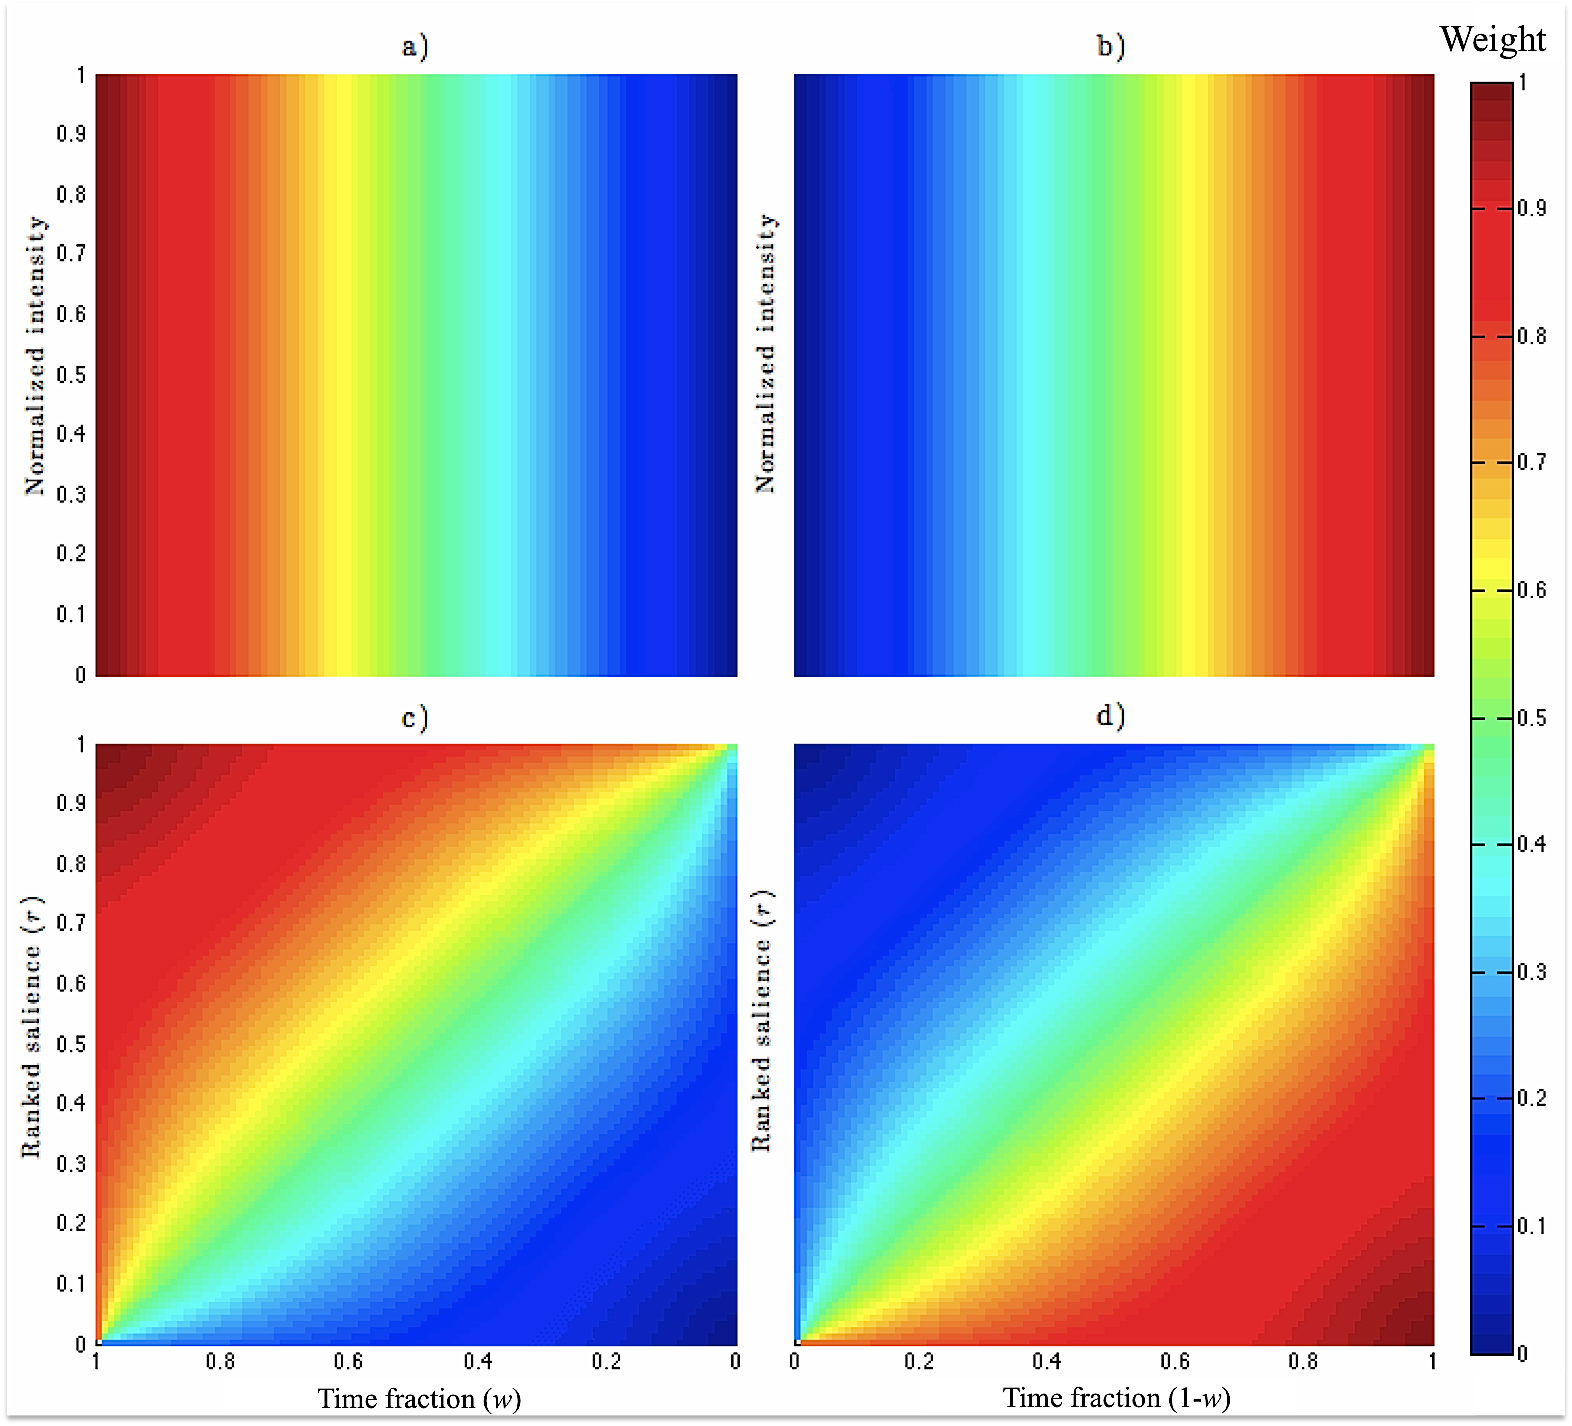
\includegraphics[width=39pc,angle=0]{f1.pdf}
%\caption{a) Linear cross-dissolve weights for extrapolation. Note that weights start at 1 regardless of intensity at 0 h and steadily decrease to 0 at maximum forecast length. 
%b) Linear cross-dissolve weights for HRRR model. Note that weights start at 0 regardless of intensity at 0 h and steadily increase to 1 at maximum forecast length. 
%c) Salient cross-dissolve weights ($w_{s}$) for extrapolation. Note that the weight of high intensity pixels (ranked saliency, $r$=$y$ axis, close to 1.0) remain high throughout the time period where low intensity pixels are dampened more quickly  
%d) Salient cross-dissolve weights ($w_{s}$) for model. The high intensity pixels ($r$ is close to 0) remain high throughout the time period.
%}
%\label{f1}
%\end{center}
%\end{figure}

%---------------------------------------------------------------------------------------------------------

\bibliographystyle{ametsoc}
\newpage
\bibliography{yunsung}

\end{document}
